\chapter{Superfici}
D'ora in avanti nel corso del capitolo sia $D \subseteq \R^2$ un dominio connesso tale che il suo interno $\mathring{D}=A$ con $A$ aperto.
\begin{definition} \label{Def: Superficie parametrica}
    Una \textbf{superficie parametrica} in $\R^3$ è un'applicazione continua $r: D \to \R^3$
    \begin{equation}
        r(u,v)=(x(u,v), y(u,v), z(u,v))
    \end{equation}
\end{definition}
Una superficie parametrica è anche descritta tramite le proprie \textit{equazioni parametriche}
\begin{equation}
    r: \begin{cases}
        x=x(u,v)\\
        y=y(u,v)\\
        z=z(u,v)
    \end{cases}
    \qquad (u,v) \in D
\end{equation}
\begin{definition} \label{Def: Sostegno di una superficie}
    Si dice \textbf{sostegno di una superficie} l'insieme $S=r(D)$
\end{definition}
In realtà una superficie propriamente detta è la coppia data da una sua parametrizzazione e il suo sostegno.\\
Inoltre, come per le curve, è possibile parlare di riparametrizzazioni di una superficie. Tuttavia, tale discorso non verrà approfondito.
\begin{definition} \label{Def: Superficie di classe C^k}
    Una superficie $r$ è detta di classe $\mathbf{C^K}$ se $r \in C^k(D)$.
\end{definition}
\begin{definition} \label{Def: Superficie semplice}
    Una superficie $r$ si dice \textbf{semplice} se $r|_A$ è iniettiva e $r(A) \cap\ r(D)= \emptyset$
\end{definition}
\begin{definition} \label{Def: Superficie regolare}
    Una superficie $r: D \to \R^3$ è detta \textbf{regolare} se essa è una superficie semplice di classe $C^1(D)$ tale che
    \begin{equation}
        J_r(u,v)= \begin{pmatrix}
            \frac{\partial x}{\partial u}(u,v) & \frac{\partial x}{\partial v}(u,v)\\
            \frac{\partial y}{\partial u}(u,v) & \frac{\partial y}{\partial v}(u,v)\\
            \frac{\partial z}{\partial u}(u,v) & \frac{\partial z}{\partial v}(u,v)
        \end{pmatrix}
    \end{equation}
abbia rango 2 per ogni $(u,v) \in \mathring{D}$
\end{definition}
\begin{definition}
    Sia $(\overline{u}, \overline{v}) \in D$ tale che $\rank(J_r(\overline{u}, \overline{v}))< 2$, allora esso è detto \textbf{punto singolare}
\end{definition}
Si può pertanto notare che la nozione di regolarità garantisce che $\tfrac{\partial r}{\partial u} (u,v)$ e $\tfrac{\partial r}{\partial v} (u,v)$ siano linearmente indipendenti per ogni $(u,v) \in \mathring{D}$. Ciò ha come conseguenza che sia ben definito il piano tangente a $S=r(D)$ in $r(u,v)$.
\begin{definition} \label{Def: Piano tangente ad una superficie}
    Sia $S$ una superficie regolare avente una parametrizzazione $r: D \to \R^3$ e sia $(u_0,v_0) \in \mathring{D}$. Allora si dice \textbf{piano tangente} a $(u_0, v_0)$ il piano definito da 
    \begin{equation}
        \Span\left\{\frac{\partial r}{\partial u} (u_0,v_0), \frac{\partial r}{\partial v} (u_0,v_0)\right\}
    \end{equation}
\end{definition}
Rispetto a tale fatto si può dire di più. Si prenda una curva regolare $\gamma$ contenuta in $D$. Si può verificare che $r$ trasforma $\gamma$ in una curva regolare $\Tilde{\gamma}:[a,b] \to S \subseteq \R^3$ di equazioni parametriche
\begin{equation}
\Tilde{\gamma}(t)= \begin{cases} 
x= x(\gamma_1(t), \gamma_2(t))\\ 
y= y(\gamma_1(t), \gamma_2(t))\\
z= z(\gamma_1(t), \gamma_2(t))
\end{cases}
\qquad t \in [a,b]
\end{equation}
Poiché $\gamma$ è regolare, anche $\Tilde{\gamma}$ è di classe $C^1$ su $[a,b]$ e in particolare
\begin{equation}
    \Tilde{\gamma}'(t)\overset{\ref{Teo: Derivata composta di f. vettoriali}}{=}
        \begin{pmatrix}
            \frac{\partial x}{\partial u}(\gamma_1,\gamma_2) & \frac{\partial x}{\partial v}(\gamma_1,\gamma_2)\\
            \frac{\partial y}{\partial u}(\gamma_1,\gamma_2) & \frac{\partial y}{\partial v}(\gamma_1,\gamma_2)\\
            \frac{\partial z}{\partial u}(\gamma_1,\gamma_2) & \frac{\partial z}{\partial v}(\gamma_1,\gamma_2)
        \end{pmatrix}
        (\gamma_1', \gamma_2') = \frac{\partial r}{\partial u}(\gamma(t))\gamma_1'(t) + \frac{\partial r}{\partial v}(\gamma(t))\gamma_2'(t)
\end{equation}
si può dedurre che per ogni $t \in [a,b]$ $\Tilde{\gamma}'$ è combinazione lineare dei generatori linearmente indipendenti del piano tangente. Ciò significa che il piano tangente contiene tutte le tangenti in $r(u,v)$ a curve regolari con sostegno in $S$ passanti per $r(u,v)$.
\begin{definition} \label{Def: Versore normale a una superficie}
    Sia $S$ una superficie regolare in ogni punto $(u,v)\in \mathring{D}$ di parametrizzazione $r$. Allora su $S$ è ben definito il \textbf{versore normale} a $S$ in $P=(u_0,v_0) \in \mathring{D}$ ed è dato da
    \begin{equation}
        \nu(P)= \pm \frac{\frac{\partial r}{\partial u} \wedge \frac{\partial r}{\partial v}}{\left|\frac{\partial r}{\partial u} \wedge \frac{\partial r}{\partial v}\right|}
    \end{equation}
\end{definition}
    In aggiunta, poiché il piano tangente è per definizione ortogonale a $\nu(P)=(\nu_1(P), \nu_2(P), \nu_3(P))$, la sua equazione è:
    \begin{equation} \label{Eq: Equazione piano tangente a una superficie}
        \nu_1(P)(x-x(u,v))+ \nu_2(P)(y-y(u,v))+\nu_3(P)(z-z(u,v))=0
    \end{equation}
\section{Superfici orientabili}
Sia $r: D=\overline{A} \to \R^3$ una superficie regolare. Allora si dice $S_0:= r(A)$ \textbf{parte interna} di $S$. Inoltre, per regolarità di $S$ è ben definita e continua rispetto a $(x,y,z)$ la funzione
\begin{equation}
    \nu: P \in S_0 \subseteq \R^3 \mapsto \nu(P) \in \R^3
\end{equation}
\begin{oss}
    La continuità di $\nu$ discende dal teorema di invertibilità globale, di cui però non si è parlato durante il corso.
\end{oss}
\begin{definition} \label{Def: Superficie orientabile}
Una superficie $S$ si dice \textbf{orientabile} se $\nu$ può essere estesa con continuità da $S_0$ a $S$. In maniera equivalente, $S$ si dice orientabile se per ogni curva chiusa continua $\varphi: [a,b] \to S$ si ha che
\begin{equation}
    \lim_{t \to b^-}{\nu(\varphi(t))}=\nu(\varphi(a))
\end{equation}
\end{definition}
\begin{example} [Nastro di Möbius]
    Si mostri un esempio di superficie non orientabile.
\begin{figure}[H]
     \centering
     \begin{minipage}{0.4\textwidth}
     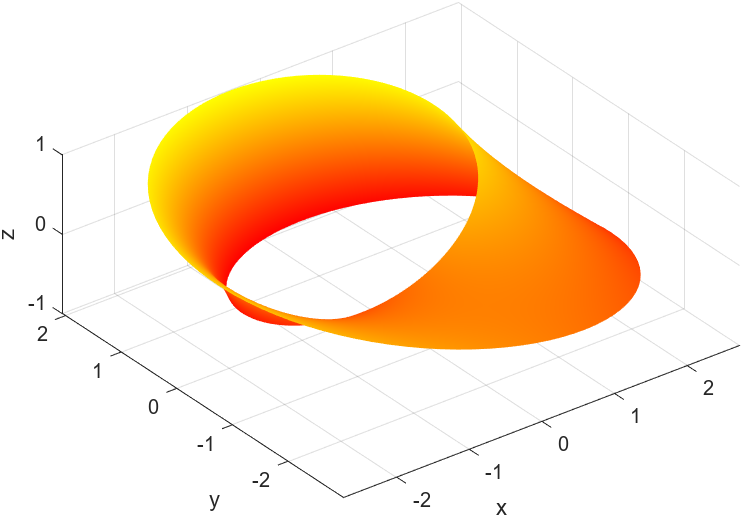
\includegraphics[width=\textwidth]{Capitoli/Capitolo6/Nastro di Moebius.png}
     \end{minipage}
     \begin{minipage}{0.55\textwidth}
        Una possibile parametrizzazione di tale superficie può essere
        \begin{equation*}
            r(u,v)= \begin{cases}
                \left(2-v \sin\left(\frac{u}{2}\right)\right) \sin(u)\\
                \left(2-v \sin\left(\frac{u}{2}\right)\right) \cos (u)\\
                v \cos\left(\frac{u}{2}\right)
            \end{cases}
        \end{equation*}
    con $u \in [0, 2\pi], v \in [-1,1]$
     \end{minipage}
 \end{figure}
 Il vettore normale di tale superficie è dato da
 \begin{equation*}
     \frac{\partial r}{\partial u} \wedge \frac{\partial r}{\partial v} = \left( \frac{1}{4}v- \frac{1}{2} \cos u - \frac{1}{4} v \cos 2u - \sin \right)
 \end{equation*}
 \begin{figure}[H]
     \centering
     \begin{minipage}{0.5\textwidth}
 In particolare, studiando i punti in cui $v$ sia nullo si ha che
 \begin{align*}
     &\lim_{u \to 0^+} \nu (u,0) = (0,-2,0)\\
     &\lim_{u \to 2\pi^-} \nu (u,0) = (0,2,0)
 \end{align*}
 e ciò non rispetta la definizione di superficie orientabile.
 \end{minipage}
 \begin{minipage}{0.3\textwidth}
     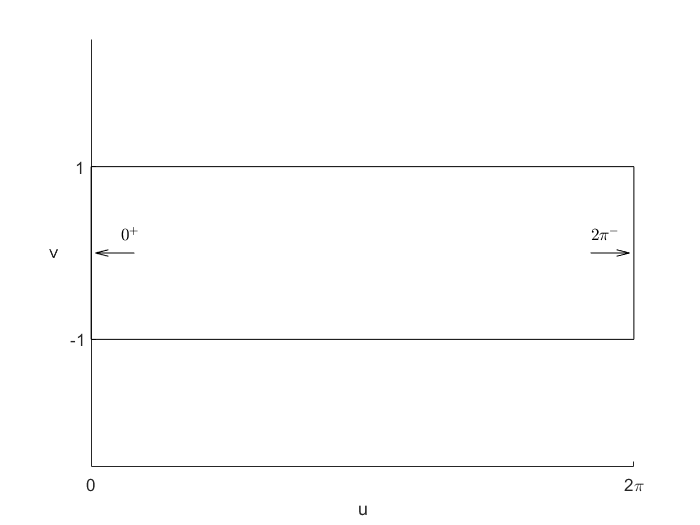
\includegraphics[width=\textwidth]{Capitoli/Capitolo6/Area per calcolo orientazione.png}
 \end{minipage}
 \end{figure}
 \end{example}
 \begin{example}
     Diversamente dal nastro di Möbius, si può osservare che i grafici di funzioni in due variabili $z=f(x,y)$ di classe $C^1$ sono superfici orientabili il cui sostegno è dato dal grafico $\mathcal{G}(f)$.
     Le equazioni parametriche della superficie sono:
     \begin{equation*}
         r(u,v)=\begin{cases}
             x= u\\
             y=v\\
             z=f(u,v)
         \end{cases}
     \end{equation*}
     Calcolando le derivate parziali ed il loro prodotto vettoriale si ha che
     \begin{equation*}
        \begin{aligned}
            &\frac{\partial r}{\partial u} = \left( 1, 0, \frac{\partial f}{\partial u}(u,v)\right)\\
            &\frac{\partial r}{\partial v} = \left( 0, 1, \frac{\partial f}{\partial v}(u,v)\right)\\
        \end{aligned}
            \qquad \Rightarrow \quad \nu(u,v)= \frac{\left(-\frac{\partial f}{\partial u}(u,v), -\frac{\partial f}{\partial v}(u,v), 1\right)}{\sqrt{1+ \left| \nabla f(u,v) \right|^2}}
     \end{equation*}
     Vale la pena notare che invertendo le variabili (ad esempio $x=v,\ y=u$) si ha un cambio di orientazione. Di conseguenza, l'orientazione dipende dalla parametrizzazione scelta.\\
     Inoltre, tramite il normale, è possibile distinguere tra "sopra" e  "sotto" o tra "dentro" e "fuori".
     \begin{figure}[H]
         \centering
         \begin{minipage}{0.4\textwidth}
         Si prenda ad esempio un paraboloide di equazione:
         \begin{align*}
             r(u,v)= \begin{cases}
                 x=u\\
                 y=v\\
                 z=u^2+v^2
             \end{cases}
         \end{align*}
        con $u \in [-1.5, +1.5],\ v \in [-1.5, +1.5]$.\\
        Calcolando, secondo le diverse convenzioni di segno, il versore normale è possibile visualizzare graficamente quanto asserito prima rispetto al "sopra" e "sotto".
     \end{minipage}
    \begin{minipage}{0.5\textwidth}
        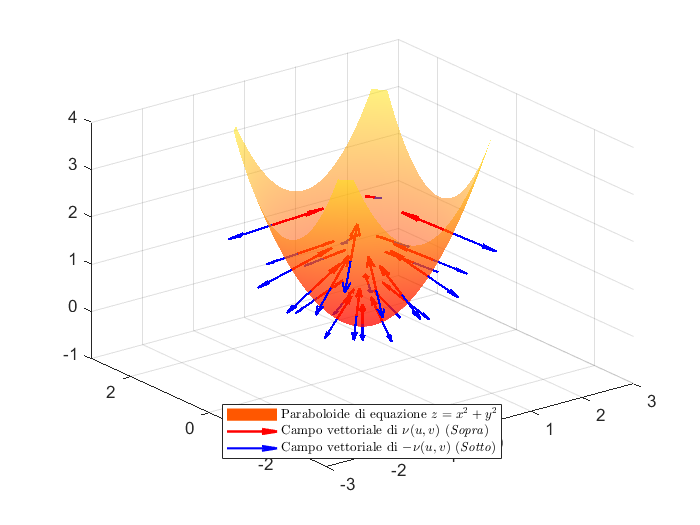
\includegraphics[width=\textwidth]{Capitoli/Capitolo6/Paraboloide.png}
    \end{minipage}
    \begin{minipage}{0.5\textwidth}
    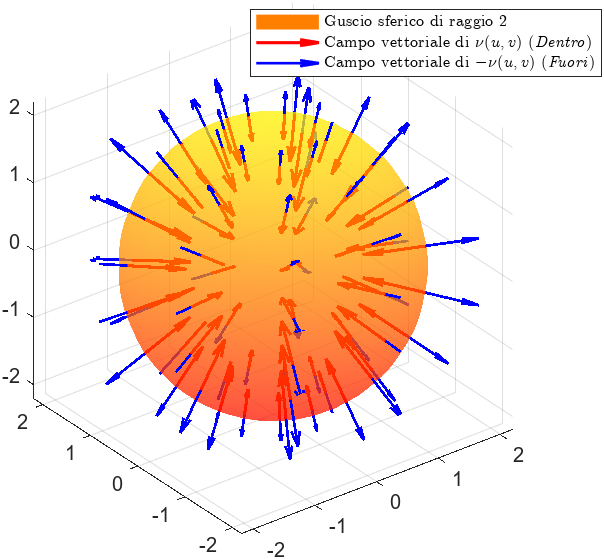
\includegraphics[width=\textwidth]{Capitoli/Capitolo6/Guscio sferico.png}
    \end{minipage}
    \begin{minipage}{0.4\textwidth}
    Discorso analogo, rispetto al "dentro" o "fuori" può essere fatto con un guscio sferico di raggio $R$ fissato. In figura $R=2$ con una superficie di parametrizzazione
    \begin{align*}
    r(u,v)=\begin{cases}
        x= R \sin u \cos v\\
        y= R \sin u \sin v\\
        z= R \cos u
    \end{cases}    
    \end{align*}
    con $u \in [0, 2\pi],\ v \in [0, \pi]$.
    \end{minipage}
    \end{figure}
 \end{example}
\section{Integrali superficiali}